\subsubsection{UC17 - Visualizzazione Beni Fattura}
\begin{figure}[h]
	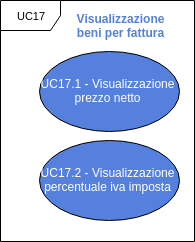
\includegraphics[width=4cm]{res/images/UC17-VisualizzazioneBeniFattura.png}
	\centering
	\caption{UC14.3 -Visualizzazione dei beni in una fatture}
\end{figure}
\begin{itemize}
	\item \textbf{Attori Primari}: azienda;
	\item \textbf{Descrizione}: l'azienda visualizza un bene nel formato fattura, ciò avviene durante la visualizzazione di una fattura in dettaglio. Per permettere all'azienda cliente di effettuare dei controlli, vengono mostrati, per ogni prodotto, prezzo netto e percentuale IVA imposta;
	\item \textbf{Scenario principale}: l'azienda visualizza una fattura in modalità dettagliata [UC16.4]. Tra le informazioni sono presenti anche i prodotti dell'ordine, dei quali vengono mostrati, oltre alle informazioni di base [UC5], anche i prezzi netti e le percentuali IVA imposte in ogni prodotto;
	\item \textbf{Inclusioni}: 
	\begin{itemize}
		\item \textbf{UC5}: per la visualizzazione di un prodotto in formato fattura sono necessari i dati base del prodotto;
	\end{itemize}
	\item \textbf{Precondizione}: il sistema ha riconosciuto l'utente autenticato come azienda, l'utente ha espresso la volontà di visualizzare una fattura in dettaglio;
	\item \textbf{Postcondizione}: l'azienda ha visualizzato tale fattura con tutti i dettagli necessari.
\end{itemize} 
\subsubsection{UC17.1 - Visualizzazione Prezzo Netto}
\begin{itemize}
	\item \textbf{Attori Primari}: azienda;
	\item \textbf{Descrizione}: l'azienda visualizza il prezzo netto di ogni prodotto presente nell'ordine relativo alla fattura che sta osservando dettagliatamente;
	\item \textbf{Scenario principale}: l'utente visualizza una fattura in dettaglio, per ogni prodotto dell'ordine relativo ne visualizza il relativo prezzo netto;
	\item \textbf{Precondizione}: il sistema ha riconosciuto l'utente autenticato come azienda, l'utente ha espresso la volontà di visualizzare una fattura dettagliata;
	\item \textbf{Postcondizione}: l'azienda ha visualizzato tale fattura, in particolare ha visualizzato i prezzi netti dei prodotti relativi all'ordine a cui si riferisce la fattura.
\end{itemize}
\subsubsection{UC17.2 - Visualizzazione Percentuale IVA Imposta}
\begin{itemize}
	\item \textbf{Attori Primari}: azienda;
	\item \textbf{Descrizione}: l'azienda visualizza la percentuale IVA imposta ad ogni prodotto presente nell'ordine relativo alla fattura che sta osservando dettagliatamente;
	\item \textbf{Scenario principale}: l'utente visualizza una fattura in dettaglio, per ogni prodotto dell'ordine relativo ne visualizza la percentuale IVA imposta;
	\item \textbf{Precondizione}: il sistema ha riconosciuto l'utente autenticato come azienda, l'utente ha espresso la volontà di visualizzare una fattura dettagliata;
	\item \textbf{Postcondizione}: l'azienda ha visualizzato tale fattura, in particolare ha visualizzato le percentuali IVA imposte ad ognuno dei prodotti relativi all'ordine a cui si riferisce la fattura.
\end{itemize}